\documentclass[10pt,a4paper]{article}
\usepackage[latin1]{inputenc}
\usepackage[english]{babel}
\usepackage{amsmath}
\usepackage{amsfonts}
\usepackage{amssymb}
\usepackage{graphicx}
\usepackage{fancyhdr}
\usepackage{lastpage}
\usepackage{multirow}

%Include and define  c code
\usepackage{listings}
\usepackage{color}
\usepackage{textcomp}
\definecolor{listinggray}{gray}{0.9}
\definecolor{lbcolor}{rgb}{0.9,0.9,0.9}
\lstset{
	language=C,
	keywordstyle=\bfseries\ttfamily\color[rgb]{0,0,1},
	identifierstyle=\ttfamily,
	commentstyle=\color[rgb]{0.133,0.545,0.133},
	stringstyle=\ttfamily\color[rgb]{0.627,0.126,0.941},
	showstringspaces=false,
	basicstyle=\small,
	numberstyle=\footnotesize,
	numbers=left,
	stepnumber=1,
	numbersep=10pt,
	tabsize=2,
	breaklines=true,
	prebreak = \raisebox{0ex}[0ex][0ex]{\ensuremath{\hookleftarrow}},
	breakatwhitespace=false,
	aboveskip={1.5\baselineskip},
  columns=fixed,
  upquote=true,
  extendedchars=true,
 frame=single,
 backgroundcolor=\color{lbcolor},
}

\oddsidemargin  -0.5cm
\evensidemargin 0.0cm
\textwidth      17.25cm
\headheight     1.0cm
\headsep		0.7cm
\topmargin      -0.5cm
\textheight		22.0cm

\pagestyle{fancy}
\lhead{Exercise 5}
\chead{EEMB1}
\rhead{\thepage\ of \pageref{LastPage}}
\lfoot{Theis Christensen\\Paulo Fontes\\Dennis Madsen}
\cfoot{Team3}
\rfoot{\today}
\renewcommand{\headrulewidth}{0.4pt}
\renewcommand{\footrulewidth}{0.4pt}
\begin{document}
\part*{EMB 2010 Team3 Exercise4}
\section{Introduction}
The job is to create a spi.c (and a spi.h) file containing two functions. A initialization of the SPI line and a transfer function.
Sending data from the master device (the LPC2478) to its slave devices (the display- and touch controllers). 
Also the goal with this exercise is to read and understand code provided by others, where changes can be done to
fit the project it should be used.
\\ \newline
In the below figure is seen how the clock is routed through the system to the ADC block. The clock value putted into the block is 28.8MHz.
\begin{figure}[h!]
   \centering
   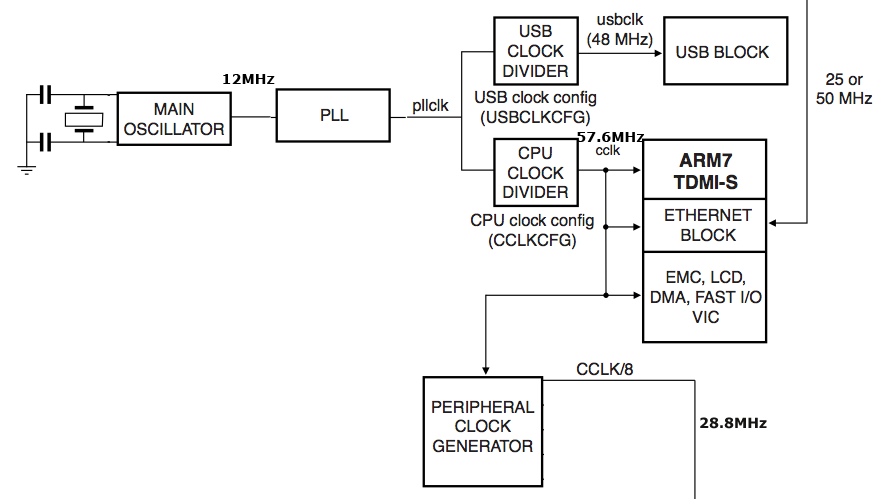
\includegraphics[width=0.7\textwidth]{peripheral_clock_gen.png}
   \caption{Peripheral clock scaling}
   \label{fig:example}
\end{figure}
\section{Initialization}

In the calib\_app.c function the SPIInit function is called with some parameters, therefore a function has been build that takes these parameters. 
The parameters are: Clock, Framesize, CPHA, CPOL, LSBF. These parameters have been chosen because of the arguments passed to the 
SPIInit function in the calibrateStart function (found in the calib\_app)
\begin{lstlisting}
	/* SSD1289 fclk max 13MHz, clk HI idle, MSB first */
	/* SPIInit(wClock, nFramesize, bCPHA, bCPOL, bLSBF)*/
	SPIInit(CLK5M, 8, 0, 1, 0);
	
	/* tsc2046:fclk max 2.5MHz, clk LO idle, MSB first
	* SPIInit(wClock, nFramesize, bCPHA, bCPOL, bLSBF)*/
	SPIInit(CLK2M5, 8, 0, 0, 0);
\end{lstlisting}

The SPIInit function takes 5 parameters, where the clock speed can be changed, the size and direction (LSB/MSB first) of the data package,
which edge is used for setting up new data and which is used to clock out data.
The display is setup to data sampling on falling edge, and other data is driven on rising edge. The touch is setup opposite, samples data on rising edge and other data 
is driven og falling edge.
\\ The pins p0.15, p0.17 and p0.18 is used as SCK, MISO and MOSI pins. Other than that p0.20 (touch) and p0.16 (QVGA) are used as Chip-select pins. 
Note that the Chip-select pins are not set in this function but has already been implemented in the project in the files: 
lcd\_driver.c and touch.c
\begin{lstlisting}
void SPIInit(short wClock, char nFramesize, char bCPHA, char bCPOL, char bLSBF){
	//1. Power: In the PCONP register set bit PCSPI.
	//Remark: On reset, the SPI is enabled (PCSPI = 1).

	//2. Clock: In PCLK_SEL0 select PCLK_SPI.
	//In master mode, the clock must be scaled down.
		//2.1: PCLKSEL0 &= ~((1<<16) | (1<<17));		//Default value CCLK/4
		//2.2: PCLKSEL0 |= (1<<16);									//CCLK
		//   PCLKSEL0 &= ~(1<<17);
		//2.3:																			//CCLK/2 = 28.8MHz
			 PCLKSEL0 |= (1<<17);
			 PCLKSEL0 &= ~(1<<16);
		//2.4: PCLKSEL0 |= ((1<<17) | (1<<16)); 		//CCLK/8
	//3. Pins: Select SPI pins and their modes in PINSEL0 to
		//SCK: P0.15  MISO: P0.17  MOSI: P0.18
			PINSEL0 |= (1<<31);
			PINSEL1 |= ((1<<3) | (1<<5));
	//4. Interrupts: Interrupts are not used

	//All SPI registers:
		//RW SPI Control Register (Master Mode)
	S0SPCR	= ((1<<2)|(bCPHA<<3)|(bCPOL<<4)|(1<<5)|(bLSBF<<6)|(nFramesize<<8));
	//S0SPSR = 0;		//RO SPI Status Register (Read Only)
	//S0SPDR = 0;		//RW SPI Data Register
	S0SPCCR = wClock;	//RW SPI Clock Counter Register
	//S0SPINT = 0;		//RW SPI Interrupt Register
}
\end{lstlisting}
The send spi function is straight forward. Data that should be to be sent is putted in the data register, whereafter the system waits for the 
\textit{transfer complete flag} to go high. The function returns the status register. If the \textit{transfer complete flag} has not been set within 
the value errorcount has counted to 10000 the function also returns (timeout).
\begin{lstlisting}
unsigned short SpiXfer(unsigned short nData){
	unsigned int errorcount = 0;

		//Put data to be sent into the data register
	S0SPDR = nData;
		//Wait for the transfer complete flag to go high
		//If it has not occured before 10000 clocs the function returns an error
	while ((S0SPSR & 0x80) == 0 && errorcount < 10000)
		errorcount++;

	return (S0SPDR);
}
\end{lstlisting}
\newpage
\section{It's alive...}
When the calibration is done, the program continue calling lcd\_test, which is a function that draws something one the screen where the screen is touched.
\begin{figure}[h!]
   \centering
   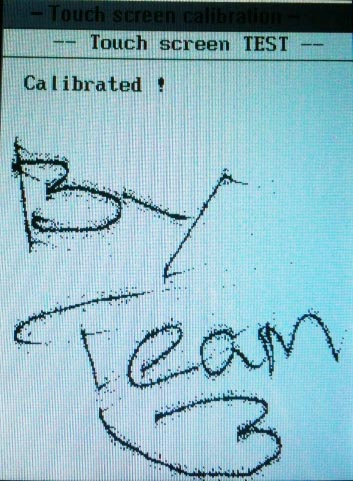
\includegraphics[width=0.4\textwidth]{lcd_test.jpg}
   \caption{Touch screen test (after calibration)}
   \label{fig:example}
\end{figure}
\textbf{ }\\ \newline
The code functions used in shortly and well described in the \textit{Exercise\_4} document provided, so no need to repetition.
\end{document}
